\chapter{The new algorithm}

% Explain what the old algorithm does
% Explain what has changed


% The new algorithm is based on 

\section{Definitions}




\section{Examples}

% When converting the sentence ``The cat is black'', from UD format to a GF format using ud2gf something happens
% 
% \begin{lstlisting}
% # gf, (gf2ud) original GF tree:
% UseCl TSim PPos (PredVP (DetCN the_Det (UseN cat_N)) (UseAP (PositA black_A)))
% # an3, (gf2ud) final annotated tree with nonlocal operations:
% @4: black black ADJ _  black_A A root
%     @2: cat cat NOUN Number=Sing  cat_N N nsubj
%         @1: the the DET _  the_Det Det det
%     @3: is be AUX Mood=Ind|Number=Sing|Person=3|Tense=Pres|VerbForm=Fin  UseAP VP cop
% 
% # ut, tree-structured UD tree:
% 4       black   black   ADJ     A       _       0       root    _       FUN=black_A
%     2   cat     cat     NOUN    N       Number=Sing     4       nsubj   _       FUN=cat_N
%         1       the     the     DET     Det     _       2       det     _       FUN=the_Det
%     3   is      be      AUX     VP      Mood=Ind|Number=Sing|Person=3|Tense=Pres|VerbForm=Fin   4       cop     _       FUN=UseAP
% 
% # ud, UD tree in CoNLLU format:
% # sent_id = gfud1000001
% # text = the cat is black
% 1       the     the     DET     Det     _       2       det     _       FUN=the_Det
% 2       cat     cat     NOUN    N       Number=Sing     4       nsubj   _       FUN=cat_N
% 3       is      be      AUX     VP      Mood=Ind|Number=Sing|Person=3|Tense=Pres|VerbForm=Fin   4       cop     _       FUN=UseAP
% 4       black   black   ADJ     A       _       0       root    _       FUN=black_A
% 
% \end{lstlisting}

\subsection{Overview of article}

We start with a UD tree

Then we assign lexical entries to each node in the tree: \lstinline|"cat" -> cat_N|, it can be several in some cases

Now we have a ud tree with a list of gf trees at each node

We start traversing the tree, depth first, when we reach a leaf, we start processing it

The main loop is: go through all the available functions and apply as many as possible and add the result to our list

When no more functions can be applied, we go to the next node in the tree.

\subsection{Example: The black cat}

For a very simple initial example, we start with the noun-phrase ``the black cat'', which has the following UD representation:

\begin{figure}[H]
    \centering
    %% the black cat
    \setlength{\unitlength}{0.2mm}
    \begin{picture}(158.0,90.0)
      \put(0.0,0.0){the}
      \put(37.0,0.0){black}
      \put(92.0,0.0){cat}
      \put(0.0,15.0){{\tiny DET}}
      \put(37.0,15.0){{\tiny ADJ}}
      \put(92.0,15.0){{\tiny NOUN}}
      \put(56.0,30.0){\oval(88.73913043478261,66.66666666666667)[t]}
      \put(11.630434782608695,35.0){\vector(0,-1){5.0}}
      \put(41.0,66.33333333333334){{\tiny det}}
      \put(74.5,30.0){\oval(49.54545454545455,33.333333333333336)[t]}
      \put(49.72727272727273,35.0){\vector(0,-1){5.0}}
      \put(59.5,49.66666666666667){{\tiny amod}}
      \put(107.0,90.0){\vector(0,-1){60.0}}
      \put(112.0,80.0){{\tiny root}}
    \end{picture}
    \caption{``The black cat'' as a UD tree}
    \label{fig:the_black_cat_ud}
\end{figure}

And we use the following abstract syntax and corresponding dependency configuration (labels-file):

\begin{verbatim}
    #fun DetCN  : Det -> CN -> NP ; det  head
    #fun ModCN  : AP  -> CN -> CN ; amod head
    #fun UseN   : N         -> CN ; head
    #fun PositA : A         -> AP ; head
    
    #cat A                        ; ADJ
    #cat Det                      ; DET
    #cat N                        ; NOUN
    
    the_Det : Det
    black_A : A
    cat_N : N
\end{verbatim}

The first step is to parse each word in the UD tree into their corresponding lexical GF functions. We use the configuration in the labels-file to convert UD-part-of-speech into their corresponding GF categories,
\begin{verbatim}
    DET -> Det
    ADJ -> A
    NOUN -> N
\end{verbatim}

which gives this tree

% TODO: Fix this so it's not so ugly
\begin{figure}[H]
    \centering
    %% the black cat
    \setlength{\unitlength}{0.2mm}
    \begin{picture}(158.0,90.0)
      \put(-30.0,0.0){the$_{Det}$}
      \put(27.0,0.0){black$_A$}
      \put(92.0,0.0){cat$_N$}
      \put(0.0,15.0){{\tiny Det}}
      \put(37.0,15.0){{\tiny A}}
      \put(92.0,15.0){{\tiny N}}
      \put(56.0,30.0){\oval(88.73913043478261,66.66666666666667)[t]}
      \put(11.630434782608695,35.0){\vector(0,-1){5.0}}
      \put(41.0,66.33333333333334){{\tiny det}}
      \put(74.5,30.0){\oval(49.54545454545455,33.333333333333336)[t]}
      \put(49.72727272727273,35.0){\vector(0,-1){5.0}}
      \put(59.5,49.66666666666667){{\tiny amod}}
      \put(107.0,90.0){\vector(0,-1){60.0}}
      \put(112.0,80.0){{\tiny root}}
    \end{picture}
    \caption{``The black cat'' as a UD tree, with GF lexicon entries inserted}
    \label{fig:the_black_cat_ud_gf}
\end{figure}

% In the case of ``the black cat sees us today'', we go down the tree until we reach ``the'', and nothing can be done there, so we continue

After this, we start traversing the tree, we go down the tree until we reach a node where all children have been processed. Since \lstinline{cat_N} has unprocessed children we keep going down and reach \lstinline{the_Det}. We look through the list of available functions and see that the only function that takes a \lstinline{Det} as an argument takes several arguments, so it can't be applied to a leaf node like this. There is nothing to be done here, so we continue.


\begin{figure}[H]
    \centering
    \subcaptionbox{``black'' as an adjective : A}[0.4\textwidth]
        {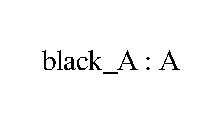
\includegraphics[scale=0.75]{thesis/figure/black_cats/black_A_gf.eps}}
    \caption{The available GF trees on the word ``black'' before the first iteration}\label{fig:black iter 0}
\end{figure}

Next we get to ``black'', with the available tree \lstinline|black_A| (\autoref{fig:black iter 0}) and here we can apply \lstinline|PositA : A -> AP ; head|, which converts an adjective into an Adjectival Phrase (AP), so now the available trees on ``black'' are
\lstinline|[black_A : A, PositA black_A : AP]| (\autoref{fig:black iter 0}), no more functions can be applied here, so we continue.

\begin{figure}[H]
    \centering
    \subcaptionbox{``black'' as an adjective : A}[0.4\textwidth]
        {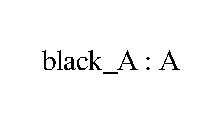
\includegraphics[scale=0.75]{thesis/figure/black_cats/black_A_gf.eps}}
    \subcaptionbox{``black'' as an adjectival phrase: AP}[0.4\textwidth]
        {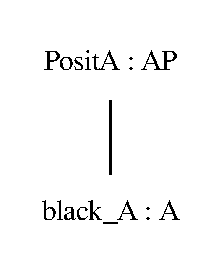
\includegraphics[scale=0.75]{thesis/figure/black_cats/black_AP_gf.eps}}
    \caption{The available GF trees on the word ``black'' after the first iteration}\label{fig:black iter 1}
\end{figure}

% A picture like 3.2, but with both the subtrees above attached to the word "black_A"

Now we are done with all the children of ``cat'', so we can start processing it. We have \lstinline|cat_N : N|. 

\begin{figure}[H]
    \centering
    \subcaptionbox{``cat'' : N}
        {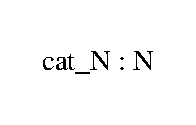
\includegraphics[scale=0.75]{thesis/figure/black_cats/cat_N_gf.eps}}
    \caption{The available GF trees on the word ``cat'' before the first iteration}\label{fig:cat iter 0}
\end{figure}

Looking through all the functions, only \lstinline|UseN : N -> CN ; head| takes an N as an argument, so that's the one that's applied, giving us \lstinline|UseN cat_N : CN|. Now we have the trees in \autoref{fig:cat iter 1}
% \begin{lstlisting}
%     cat_N : N
%     UseN cat_N : CN
% \end{lstlisting}

\begin{figure}[H]
    \centering
    \subcaptionbox{``cat'' as a noun : N}[0.4\textwidth]
        {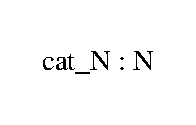
\includegraphics[scale=0.75]{thesis/figure/black_cats/cat_N_gf.eps}}
    \subcaptionbox{``cat'' as a common noun: CN}[0.4\textwidth]
        {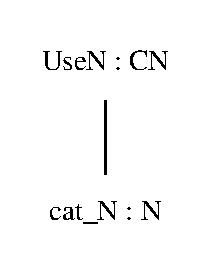
\includegraphics[scale=0.75]{thesis/figure/black_cats/cat_CN_gf.eps}}
    \caption{The available GF trees on the word ``cat'' after the first iteration}\label{fig:cat iter 1}
\end{figure}

In the next iteration we have a \lstinline|CN| available and can apply either of the functions
\begin{lstlisting}
    DetCN : Det -> CN -> NP ; det head
    ModCN : AP -> CN -> CN  ; amod head
\end{lstlisting}
Let us verify that these are possible to apply: For \lstinline|DetCN| we need a tree of type $Det$ with the $det$ ud label for the relation and indeed, the word ``the'' has the $det$ label on the relation to ``cat'' and we have the tree \lstinline|the_Det : Det| available on ``the''. Secondly we need a $CN$ at the head and since our current head is ``cat'' and we have \lstinline|UseN cat_N : CN|, that fits perfectly giving us \lstinline|DetCN the_Det (UseN cat_N) : NP|. With similar reasoning for \lstinline{ModCN}, we have ``black'' with UD-label $amod$ and one of the available trees for ``black'' is \lstinline|PositA black_A : AP| which has the correct category, which allows us to construct \lstinline|ModCN (PositA black_A) (UseN cat_N) : CN|. After this we have the trees in \autoref{fig:cat iter 2}

\begin{figure}[H]
    \centering
    \subcaptionbox{cat : N\label{cat_N}}
        {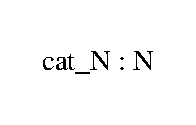
\includegraphics[scale=0.75]{thesis/figure/black_cats/cat_N_gf.eps}}
    \subcaptionbox{cat : CN\label{cat_CN}}
        {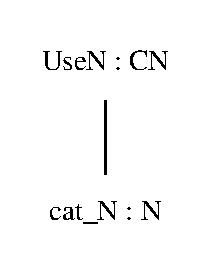
\includegraphics[scale=0.75]{thesis/figure/black_cats/cat_CN_gf.eps}}
    \subcaptionbox{the cat : NP\label{the_cat_NP}}
        {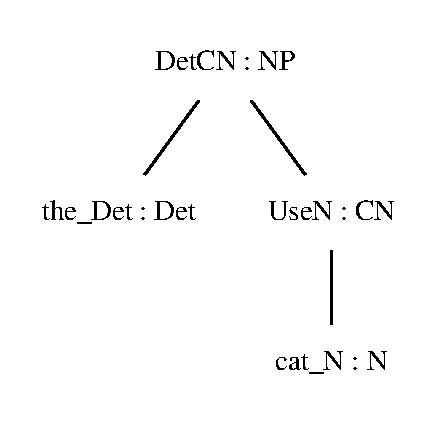
\includegraphics[scale=0.75]{thesis/figure/black_cats/the_cat_NP_gf.eps}}
    \subcaptionbox{black cat : CN\label{black_cat_CN}}
        {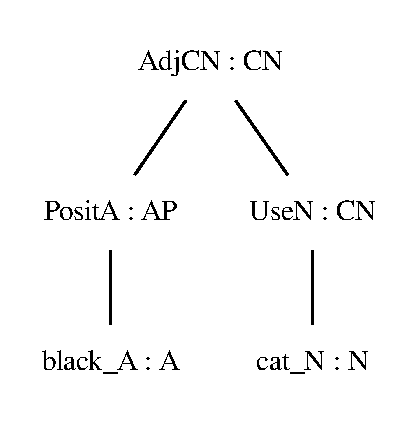
\includegraphics[scale=0.75]{thesis/figure/black_cats/black_cat_CN_gf.eps}}
    \caption{The four available trees on the word ``cat'' after the second iteration}\label{fig:cat iter 2}
\end{figure}

After this iteration we have two trees on ``cat'' which both have the same category $CN$, namely
\begin{lstlisting}
    UseN cat_N : CN
    ModCN (PositA black_A) (UseN cat_N) : CN
\end{lstlisting}
and one of them is a strict superset of the other when it comes to words covered, the first only covers ``cat'' while the second covers both ``black'' and ``cat''. This means we can prune the redundant tree \lstinline{UseN cat_N}.

\begin{figure}[H]
    \centering
    \subcaptionbox{Cat\label{ci2p:cat_N}}
        {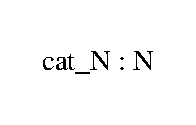
\includegraphics[scale=0.75]{thesis/figure/black_cats/cat_N_gf.eps}}
    \subcaptionbox{The cat\label{ci2p:the_cat_NP}}
        {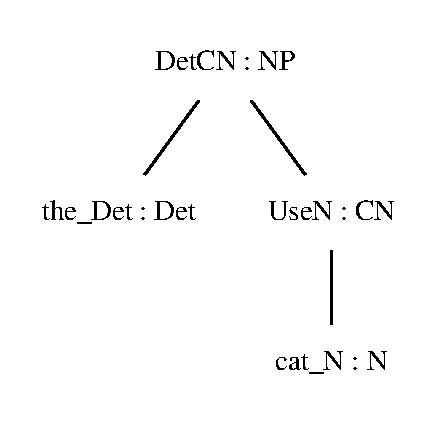
\includegraphics[scale=0.75]{thesis/figure/black_cats/the_cat_NP_gf.eps}}
    \subcaptionbox{Black cat\label{ci2p:black_cat_CN}}
        {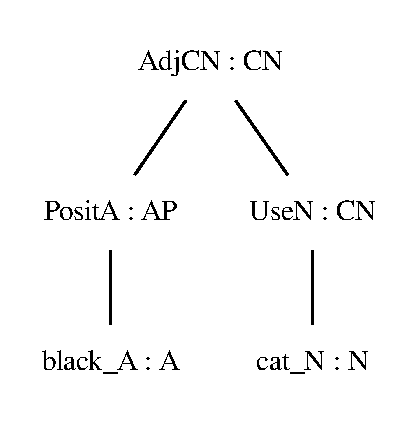
\includegraphics[scale=0.75]{thesis/figure/black_cats/black_cat_CN_gf.eps}}
    \caption{The three available trees on the word ``cat'' after the second iteration after pruning}\label{fig:cat iter 2 pruned}
\end{figure}

After this pruning, the available trees on the ``cat'' node are
\begin{lstlisting}
    cat_N : N
    DetCN the_Det (UseN cat_N) : NP
    ModCN (PositA black_A) (UseN cat_N) : CN
\end{lstlisting}
After this step, one function is still possible to apply, namely $DetCN$, which can be applied to our new $CN$ together with \lstinline{the_Det} like before, giving us
\begin{lstlisting}
    DetCN the_Det (ModCN (PositA black_A) (UseN cat_N)) : NP
\end{lstlisting}
and like before, we get multiple trees of the same category, this time of type $NP$, once again allowing us to prune the less covering tree
\begin{lstlisting}
    DetCN the_Det (UseN cat_N) : NP
\end{lstlisting}

After this no more functions can be applied at the ``cat'' node, giving us a final set of cat trees
\begin{lstlisting}
    cat_N : N
    ModCN (PositA black_A) (UseN cat_N) : CN
    DetCN the_Det (ModCN (PositA black_A) (UseN cat_N)) : NP
\end{lstlisting}

and from here we continue in a similar fashion with the rest of the sentence.

\begin{figure}
    \centering
    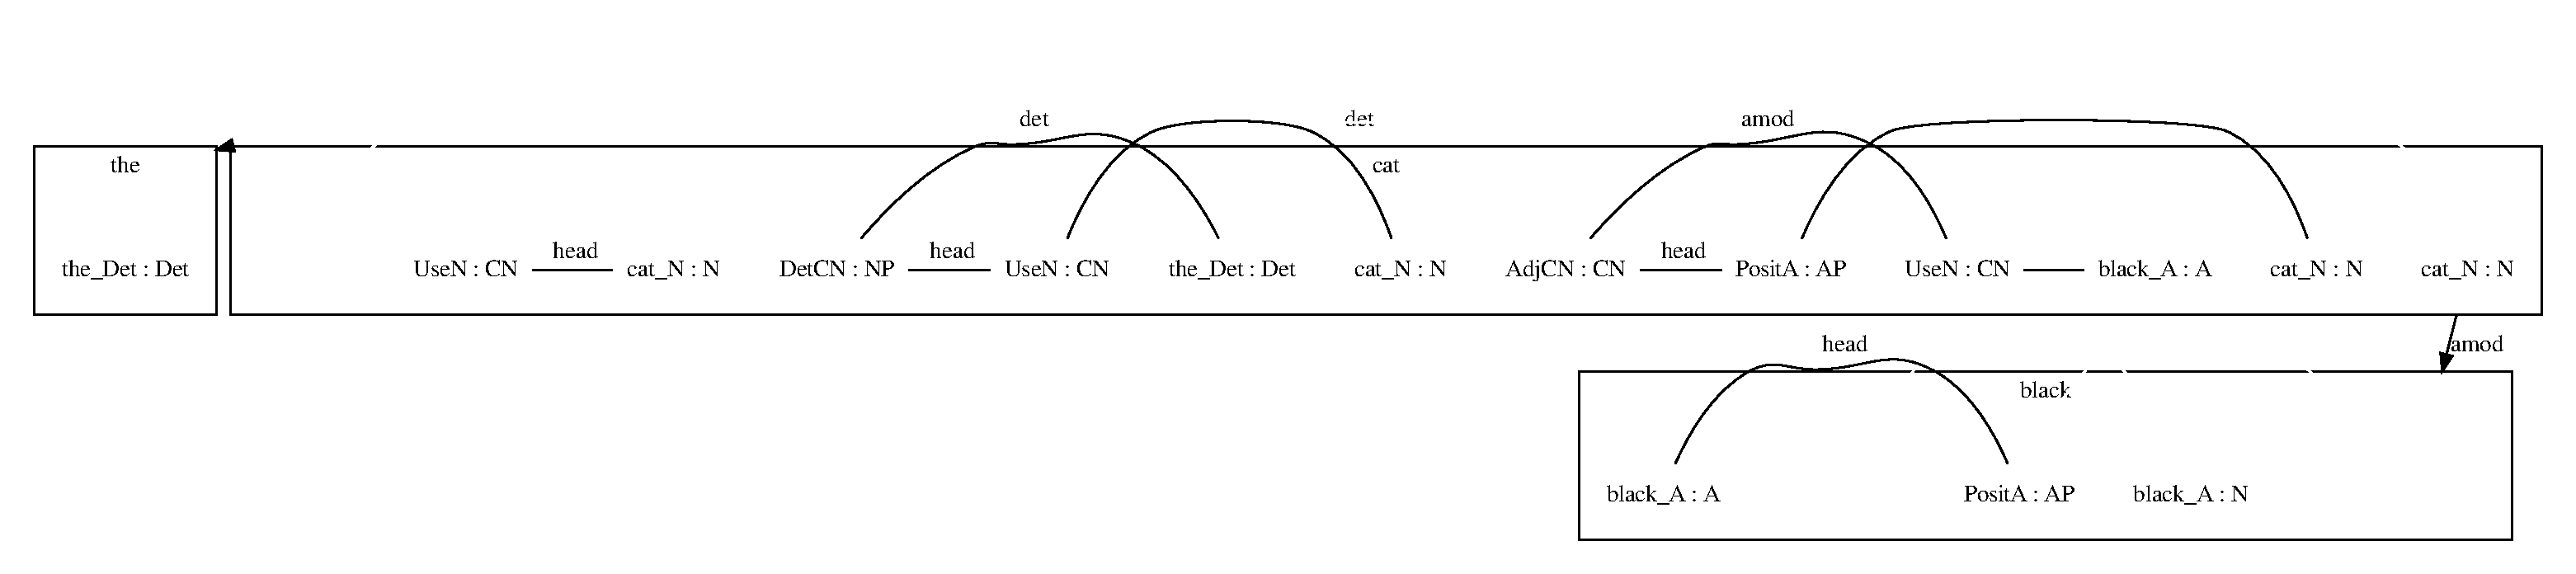
\includegraphics[width=0.7\textwidth]{figure/black_cats/he_black_cat_graph.eps}
    \caption{An overview of the nested tree, with the UD structure outside and a list of GF-trees at each node}\label{fig:final nested tree}
\end{figure}


\subsection{Differences between versions}

In the version 2 algorithm, in each iteration for a node in the UD tree (which corresponds to a word), after we have applied all possible functions and want to check if that unlocked new possible function applications, we check with \emph{all} the available trees in that node against each available function. This means that all the trees that were possible to construct in the previous iteration are still possible to construct, so we will construct them again and will need to remove the duplicates afterwards.



(issues: in some cases we can get an infinite loop if we have e.g. a function \lstinline{: A -> A})



\section{How annotations work}